\documentclass[conference]{IEEEtran}
\IEEEoverridecommandlockouts
% The preceding line is only needed to identify funding in the first footnote. If that is unneeded, please comment it out.
\usepackage{cite}
\usepackage{amsmath,amssymb,amsfonts}
\usepackage{algorithmic}
\usepackage{graphicx}
\usepackage{textcomp}
\usepackage{xcolor}
\usepackage{tikz}
\usepackage{balance}
\def\BibTeX{{\rm B\kern-.05em{\sc i\kern-.025em b}\kern-.08em
    T\kern-.1667em\lower.7ex\hbox{E}\kern-.125emX}}
\begin{document}

\title{Analyzing Network Routing Resilience: A Hybrid Approach of Face and Tree Routing}

\author{
    \IEEEauthorblockN{Georgios Karamoussanlis}
    \IEEEauthorblockA{\textit{TU Dortmund}\\Dortmund, Germany}
    \and
    \IEEEauthorblockN{Stephanie Althoff}
    \IEEEauthorblockA{\textit{TU Dortmund}\\Dortmund, Germany}
    \and
    \IEEEauthorblockN{Erik van den Akker}
    \IEEEauthorblockA{\textit{TU Dortmund}\\Dortmund, Germany}
    \and
    \IEEEauthorblockN{Klaus-Tycho Foerster}
    \IEEEauthorblockA{\textit{TU Dortmund}\\Dortmund, Germany}
}

\maketitle

\begin{abstract}
%One or two sentences providing a basic introduction to the field, comprehensible to a scientist in any discipline.
With the aim of ensuring reliable and consistent communication, network topologies need to be able to correctly and rapidly respond to potential errors. Through these responses, the connection within the network is maintained, even in the presence of faults. This is achieved through various mechanisms, known as fast failover algorithms, which are implemented in the data~plane, opposed to the slower control plane.

%Two to three sentences of more detailed background, comprehensible to scientists in related disciplines.
%- Zum Hintergrund: Bis jetzt wurde das Tree Routing häufiger benutzt, was ist aber wenn das Tree Routing Probleme bekommt bspw. mit Knoten die Fehleranfällig sind?
In this work, an established fast failover approach, which routes through trees, is extended. This extension is achieved by dividing the routing path into two parts and using both face routing and tree routing for forwarding packets.
%One sentence clearly stating the general problem being addressed by this particular study.
This is done against the backdrop that Tree Routing yields suboptimal results when the source of the routing is highly error-prone. To counteract this, this work proposes a modification of the Tree Routing by first routing through a waypoint using face routing and then utilizing tree routing.
As such, the routing is resilient to errors both at the source and destination.

%One sentence summarizing the main result (with the words “here we show” or their equivalent).
Results of this work showed in a setting of clustered failures using real world graphs, resilience can be enhanced, with a higher hop count due to utilizing the faces to circumvent early failures.
Additionally, randomized errors in randomized graphs have been demonstrated to increase resilience as well compared to the original tree routing algorithm.


%Two or three sentences explaining what the main result reveals in direct comparison to what was thought to be the case previously, or how the main result adds to previous knowledge.
%- Detaillierter was das Ergebnis aussagt.

%One or two sentences to put the results into a more general context. 

%Two or three sentences to provide a broader perspective, readily comprehensible to a scientist in any discipline, may be included in the first paragraph if the editor considers that the accessibility of the paper is significantly enhanced by their inclusion. Under these circumstances, the length of the paragraph can be up to 300 words. (This example is 190 words without the final section, and 250 words with it)
%- Was der Einsatz von dem Facerouting bringen könnte für die Zukunft und warum man das machen sollte.
\end{abstract}

\begin{IEEEkeywords}
    fast failover routing, routing, face routing, tree routing
\end{IEEEkeywords}

\section{Introduction}
\subsection{Motivation}
In today's digital society, we increasingly rely on communication networks. Many applications, 
such as i.e. financial transactions or medical software, require a high availability of service. 
Network outages are causing a degradation in service quality \cite{blackHolesInternetHubble} 
and can lead to high costs \cite{surveyInternetOutages}. 
However, networks have been expanded significantly in size over the years, which leads to a 
corresponding increase of data traffic.
Consequently, the likelihood of packets encountering failures during transmission has grown~\cite{measurementsFailuresDataCenters}.
In the modern era, managing failures of communication networks has, therfore, become increasingly~critical. 

It is essential for networks to be equipped to handle node failures and to provide 
alternative paths ensuring that packets reach their intended destinations.
Due to stringent availability requirements, local fast rerouting algorithms are used within 
the data plane in many communication networks~\cite{DBLP:journals/comsur/ChiesaKRRS21}, which are known to operate at timescales several orders 
of magnitude faster than the control plane~\cite{DBLP:conf/nsdi/LiuPSGSS13}.

\subsection{Background}
Current methods for local fast failover algorithms, which are widely used in many networks today, 
primarily utilize edge-disjoint paths to create alternative routes~\cite{only-edp1,only-edp2}. 
We refer to the survey of Chiesa et al.~\cite{DBLP:journals/comsur/ChiesaKRRS21} for a general overview.
Further research has shown that the use of tree routing can further enhance resilience \cite{tree}.
In this approach, the edge-disjoint paths are extended into trees, which are then used for routing packets through the network.
Trees are especially suited to this approach, as one can implement local fast failover routing in the nodes by traversing them in a depth-first search (DFS), where failed edges are simply \emph{skipped}~\cite{DBLP:conf/apocs/FoersterHPST21} in the local DFS traversal.
Notwithstanding, using trees brings the disadvantage that routing may be prematurely terminated when 
frequent errors occur at the root, as the path diversity is concentrated at the destination neighboring the leaf~nodes.

However, this approach cannot be directly turned into a double-tree structure, protecting both source and destination: when routing from a leaf to the destination, the packet never needs to return, as the packet has reached its intended target.
But, when returning to the source, using the local DFS-traversal approach is problematic, as connecting the source to the tree turns the routing structure into a non-tree planar graph, where resilience to failures is hard to achieve~\cite{DBLP:conf/apocs/FoersterHPST21,DBLP:conf/dsn/FoersterHPST22}.

Still, upon taking a closer look, one does not need to perform arbitrary routing in this double-tree, as we are only interested in reaching the destination from the source, and hence we can take inspiration from classic face routing~\cite{facerouting2, facerouting}.
 In this setting, the graph is divided into so-called ``faces'' and routing is based on their geometric and geographic properties.
 Even though face routing usually requires non-trvial state~\cite{DBLP:journals/comsur/CadgerCSM13} in the packets or nodes, which is undesirable in high-performance networks, we in this paper propose to simply route along the outer face to realize such a double-tree aproach, as routing along the outer face is compatible with zero-state local fast failover algorithms~\cite{DBLP:conf/apocs/FoersterHPST21,DBLP:conf/dsn/FoersterHPST22}.

\subsection{Contributions}
The present work analyzes whether the integration of face routing can improve fast failover routing in the form of tree routing.
In this context, a demand first traverses from its source to a checkpoint using face routing and is then routed to the destination using tree routing.
We denote this hybrid approach as  $One Tree Checkpoint$.
%The following hybrid approach will be referred to as $One Tree Checkpoint$.

To this end, we present a formal concept how face routing can be integrated into the context of fast failover routing for the example of tree routing.

We show in Python-based simulations that such a hybrid approach can increase resilience to link failures, for both clustered failures in real-world graphs and random failures in random graphs. 
Nonetheless, the higher resilience comes at the cost of increased hop count, as the increased path diversity, leading to better routing success, comes at the cost of longer routes post-failures.



\subsection{Organization}
The work is structured as follows: Section~\ref{Model} introduces the model and Section \ref{Concept} discusses the concepts, including both the precomputation and routing processes. Section \ref{evaluation} presents the evaluation, analyzing the resilience and hops of the various approaches. Finally, Section~\ref{conclusion} summarizes the work and Section \ref{outlook} provides an outlook on further improvements that could be made to the hybrid use of face and tree routing.
 
\section{Model}
\label{Model}
We consider networks modeled as undirected graphs $G = (V,E)$. 
For routing packets in the network, static local forwarding rules are implemented at each node for every possible combination
of source $s \in V$ and destination $d \in V$. These forwarding rules 
decide about the used outgoing edge based on the information in the
packet header, as well as the incoming port the packet was sent from. It is not allowed to modify the 
packet header to add additional information. The forwarding rules have to be installed at each node
in advance (while the failures are unknown yet). After implementing the forwarding rules, a random 
set of edges $F \subseteq E$ fails, hence the packet has to be routed
through the Graph $G' = (V, E \setminus F)$ only utilizing the previously installed forwarding rules.

Generally a forwarding pattern is called $r$-resilient, if for any set $F \subseteq E$ with $|F| = r$ 
and any source-destination pair $s,d \in V$, where $s$ and $d$ are still connected in $G'$,
packets from $s$ can still reach the destination $d$ while only following the rules of the forwarding pattern. In 
this work, we heuristically check
if a packet still reaches the destination node under random edge failures, applying our strategy, and using 
resilience to describe the probability
of the packet reaching its destination under a given failure set. A more detailed description of the used
metrics is given in Section~\ref{evaluation}.

\section{Concept and Model}
\label{Concept}
In this section the concept of connecting face routing with tree routing is described in detail. Each step 
of Fig.~\ref{conceptFigure} is referenced in the corresponding following sections. 
In the figure, arrows are shown under each step to indicate the direction in which each respective phase 
operates.
The framework \cite{fast-failover-og}, which is based on the work~\cite{casa}, has been extended in the 
present work. This is a corresponding model to~\cite{casa}, which describes the graph structures. A 
comparable model can also be found in the following work \cite{tree}.
Therefore, the model of the trees used for routing in Sections \ref{precompTree} and \ref{routingTree} 
consists of unidirectional edges to maintain the internal structure of the trees and preserve parent-child 
relationships.
The concept is encapsulated in the implementation of the $OneTreeCheckpoint$ algorithm, which will be detailed 
further in the following sections.
In the other steps of the concept, the deployed structure consists of bidirectional edges.
%The code of this concept's implementation can be found in the repository \cite{my-repo}.

\begin{figure}[t]
\centering
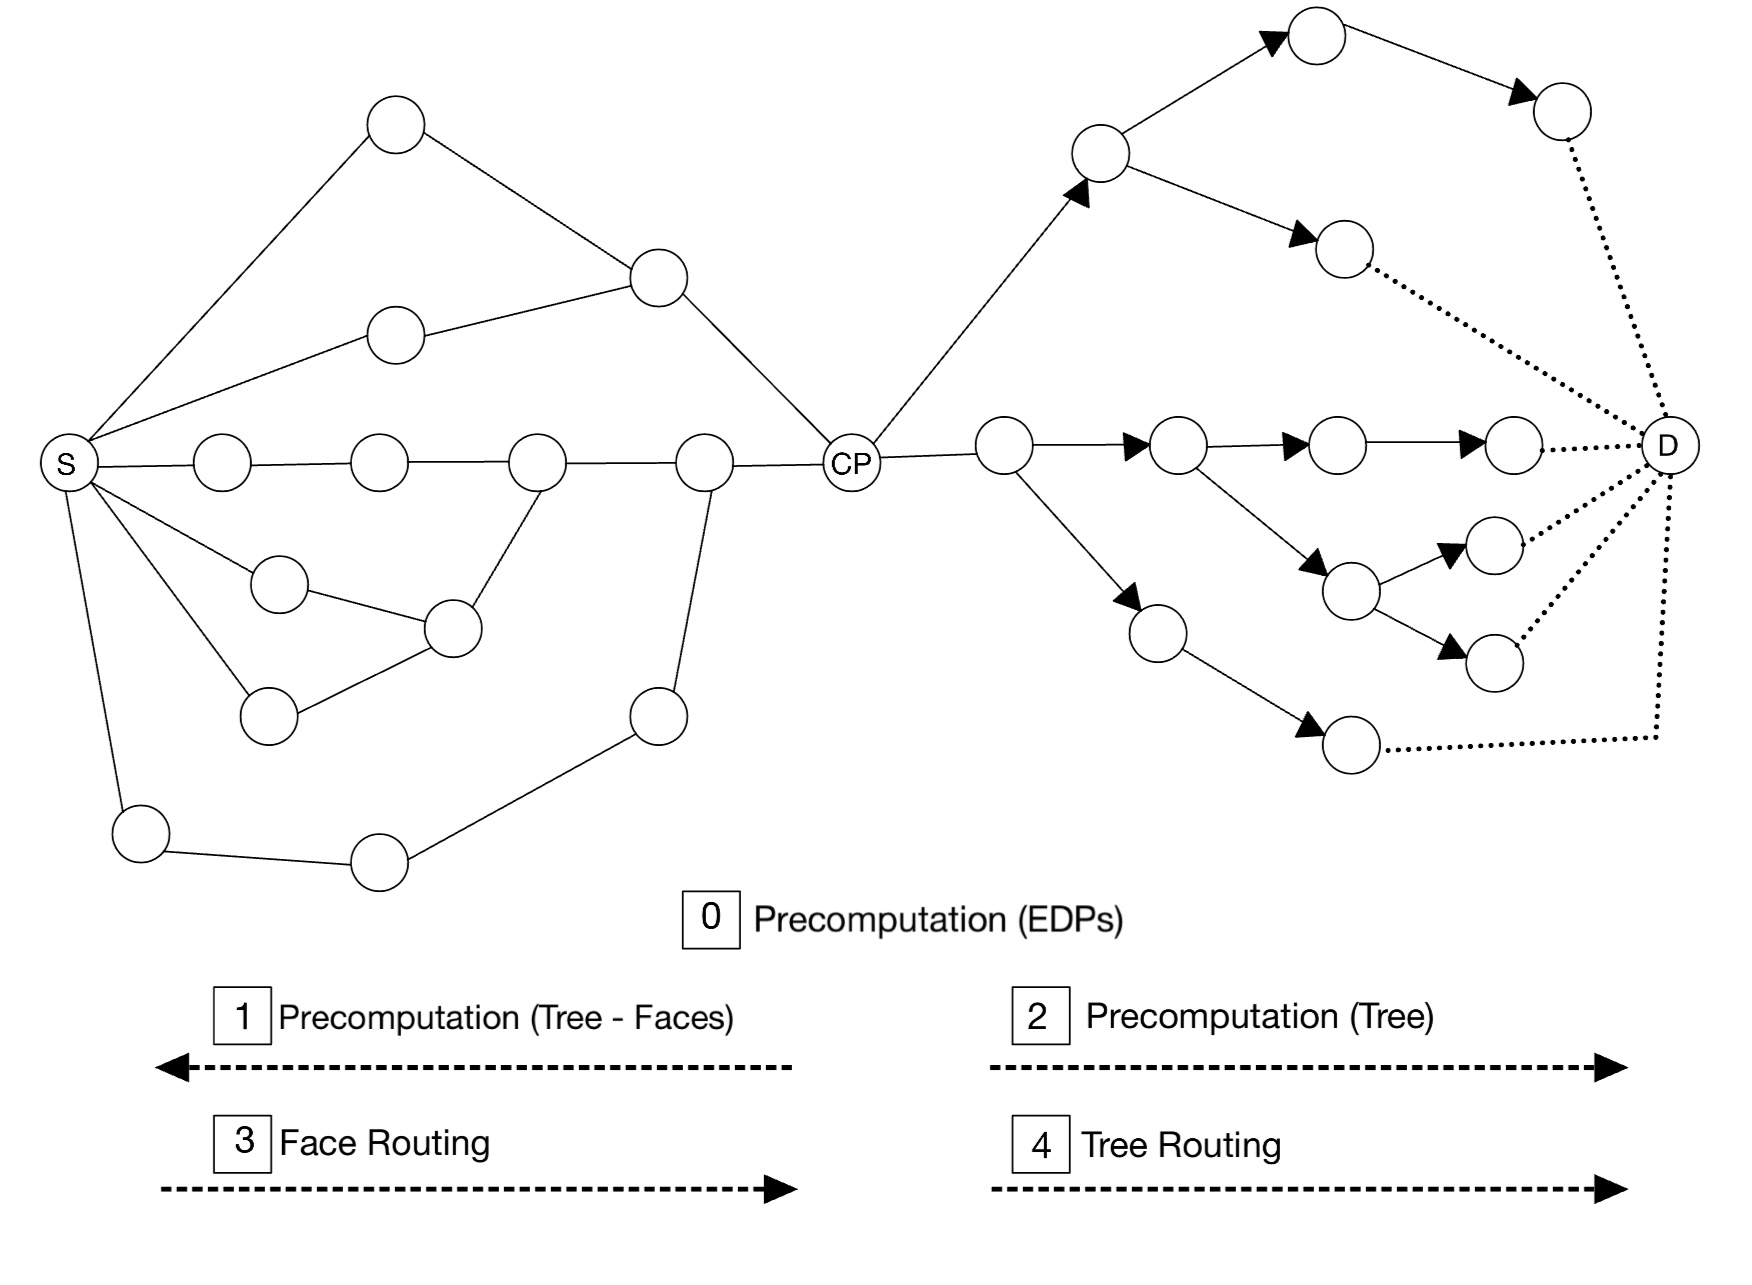
\includegraphics[scale=0.3]{figures/concept(1).jpeg}
\caption{Example graph demonstrating the step-wise implementation of the Hybrid Approach of Face and Tree Routing}
\label{conceptFigure}
\end{figure}

\subsection{Precomputation}
\label{precomputation}
In the precomputation phase, preparations are made and the underlying structures are created, which form the basis for the routing rules of the routers. This precomputation consists of three steps, which are shown in Fig.~\ref{conceptFigure} as \fbox{0}, \fbox{1}, and \fbox{2}. The precomputation fills the entries of the routing tables by building the structures of each step for every source ($s$) and destination ($d$) pair.

\subsubsection{EDPs}
Before face and tree structures are created, the edge-disjoint paths (EDPs) need to be found in step \fbox{0}.
For a given ($s$,$d$)-pair the edge-disjoint paths describe paths from $s$ to $d$ such that no two paths share an edge.
First the longest EDP is found in order to choose the checkpoint ($cp$) as a safe node for routing through.
In the current state of the algorithm, the $cp$ is the node that lies halfway through the longest EDP.
After choosing $cp$, it is used to find the remaining two EDPs in order to use them as the foundation for the structures in Section \ref{precompTree} and \ref{precompFace}.
This is done by finding the longest EDP between $s$ and $cp$ for step \fbox{1}.
Similar for step \fbox{1} the longest EDP between $cp$ and $d$ is used for step \fbox{2}.

\subsubsection{Tree}
\label{precompTree}
The underlying structures of both steps \fbox{1} and \fbox{2} are trees, that are generated by expanding the longest EDP.
In contrast to the structure of \fbox{1}, the tree in \fbox{2} is expanded to a planar structure with faces, which is described in Chapter \ref{precompFace}. 
The first tree build, expands the EDP in the direction of $cp$ to $s$.
The direction was chosen to address the issue of having too many faulty edges at the source. This leads to a multitude of leaves at the source, all of which serve as entry points into the routing structure.
The second tree expands the EDP in the direction of $cp$ to $d$.
At the beginning of the tree building algorithm, the tree consists of the longest EDP as previously described.
After that, the algorithm iterates over the current tree nodes and adds its neighboring nodes to the tree along with the corresponding edges, which not already exist in the tree.
These iterations will be terminated once no further edges can be inserted into the tree.
Next comes the pruning of the tree, as it contains paths that are not leading to the destination. The pruning function will be called repeatedly until no more nodes can be removed from the tree.
In every call of this pruning function, leaves are removed if they don't have a connection to $d$ in the topology.
At the last part of the algorithm, each node gets a rank, which describes the order in which the routing has to choose its next hop.
For this part a ranking function assigns ranks to the nodes of the tree, starting from the leaves.
A rank reveals the information about how many edges need to be traversed from the respective node to reach the destination.
A special ranking is needed for the rankings of the EDP nodes, since they need to be traversed~first.

\subsubsection{Faces}
\label{precompFace}
Since the routing of step \fbox{3} starts at $s$ and ends at $cp$, the reversed tree structure build in step \fbox{1} needs to be changed. 
This adjustment is needed due to the intricate nature of routing within a tree structure, particularly when navigating from leaf nodes towards the root, relying solely on localized information available at each node.
In order to route on this tree starting from the leaves, face routing is chosen as the concept of routing to the checkpoint. 
Being able to use face routing and find the faces of a graph, implies that the graph is planar. 
This is given by the definition of a graph represented as a tree \cite{treeIsPlanar}.
Conducive to route from $s$ to $cp$, the source gets connected to the leaves of the structure and coordinates get added to each node of the structure, representing a planar topology.
Following the coordinates of each node, the faces of the structure need to be determined.
The algorithm determines the faces of a planar graph by traversing each node and examining the half-edges emanating from that node. 
New faces are identified by visiting neighboring nodes starting from a node until a closed path is formed.

\subsection{Routing}
The routing is divided into 2 sections (Sections \ref{routingTree} and \ref{routingFaces}), as shown in Fig.~\ref{conceptFigure}. The routing scheme changes as soon as the packet to be sent has arrived at $cp$. This is due to the change in the underlying structure, which was described in Chapter \ref{precomputation}.
Before using the structure provided by the precomputation, packets are routed along the EDPs, which span from $s$ to $d$.
In case the routing via the EDPs fails, the packet then first passes through a planar structure with faces \fbox{3} and then through a tree structure \fbox{4}.


\subsubsection{Face Routing}
\label{routingFaces}
Face routing describes the first part that the packet traverses on its complete route to the destination. It is first routed from $s$ to $cp$. 
The idea of the face routing algorithm is similar to \cite{facerouting}.
Since the structure created in Chapter \ref{precompFace} is planar and the faces have been determined, the following section explains how to route in any face in order to get to the next face or to find the destination directly.
An example of the face routing  algorithm is shown in Fig. \ref{faceRoutingExample}. 
Three variables are given in this Figure, which include the Entry Point ($EP$), from where the routing starts in the current face, the Destination ($D$), and the Intersection Point ($IP$), which represents the intersection point between the imaginary edge ($EP$, $D$).
In the first phase of routing, the demand follows the green arrows. At each edge, it is checked whether it intersects with the imaginary edge. If such an intersection exists, it is further checked if this intersection is the one closest to the destination and is stored. This process is repeated until an invalid edge is encountered, causing the routing to backtrack, or a loop within the face is completed.
Next, the packet follows the blue path to the node of the previously determined nearest $IP$ and transitions to the next face. At this point, this process is repeated until the packet encounters $D$ in the first pass.


\begin{figure}[t]
    \centering
    \raisebox{0pt}[\height][\depth]{\hspace*{-1cm}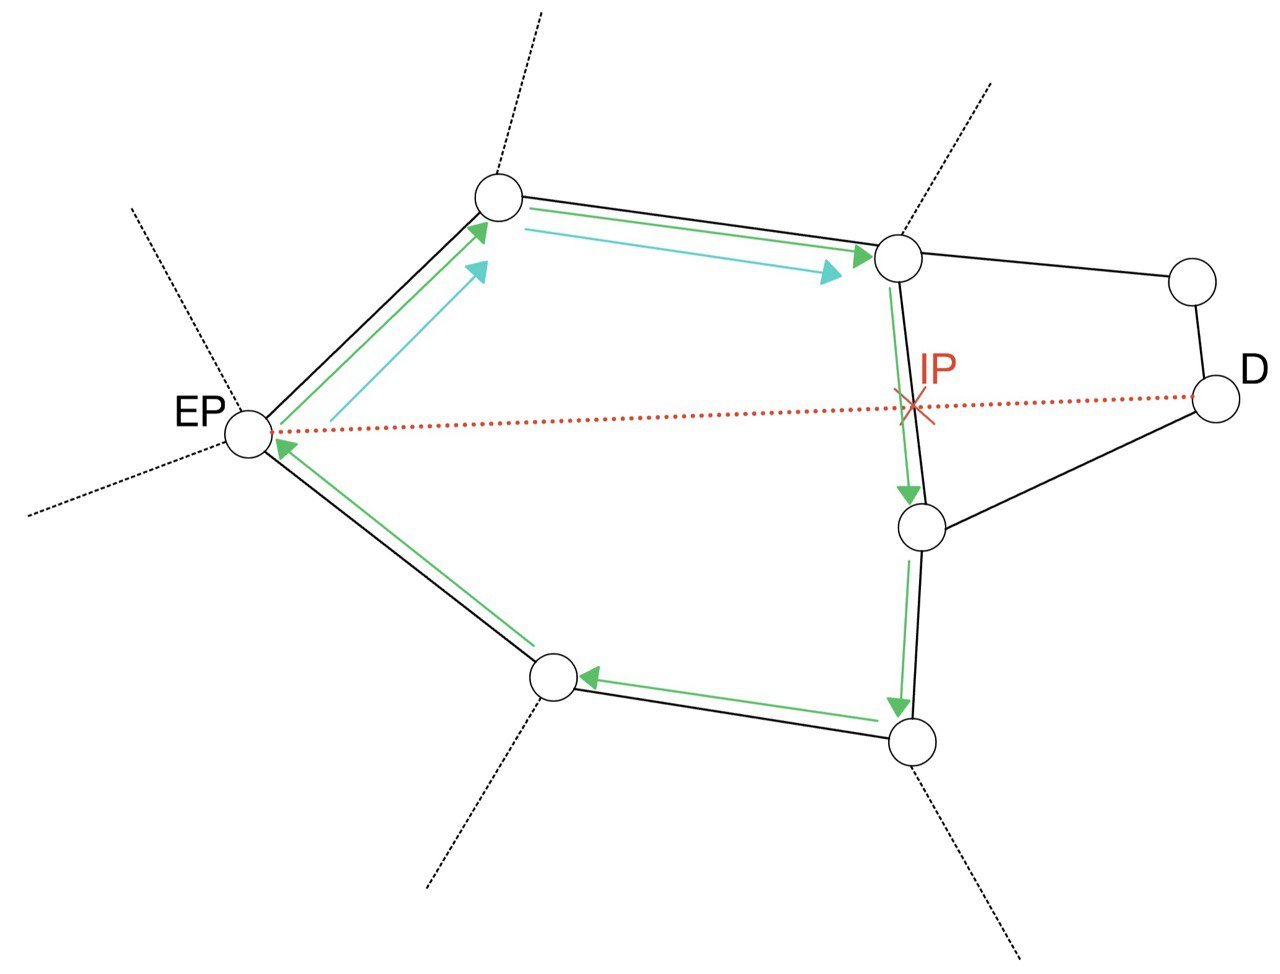
\includegraphics[scale=0.19]{figures/faceroutingExample.jpg}}
    \caption{Example of Face Routing used in step \fbox{3}. \textcolor{green}{First path} is searching for the \textcolor{red}{intersection point (IP)} and \textcolor{blue}{second path} is traversing to the closest intersection from the entry point (EP) of the face}

    \label{faceRoutingExample}
\end{figure}

\subsubsection{Tree Routing}
\label{routingTree}
Tree routing describes the second part that the packet goes through on its complete path to the destination. In this part, it is ultimately routed from $cp$ to $d$.

First, routing follows the previously edge-disjoint paths. This is ensured by prioritized ranking.
The lower the rank of a node, the higher its priority.
Assuming that all EDPs contain a faulty edge, the routing begins via the tree. This is divided into sections, which correspond to the type of port through which the packet arrives at any node ($A$) of Fig. \ref{treeRoutingExample}.

When the packet arrives through the incoming edge of the parent node, it indicates that node $A$ is being visited for the first time. Therefore, the optimal child ($B$) with the lowest rank is selected first, the packet is forwarded there, and the process is repeated.

If the packet returns through the child node $B$ because all outgoing edges there might have failed, it means that another child must be selected. For this, all outgoing edges from $A$ are sorted by their ranks, and it is checked which child has the next higher rank compared to $B$. In this case, it would be $C$. This process is similar if the packet is sent back from node $C$ to node $A$.

In the last case, the packet arrives back at $A$ from $D$. This means that the child with the highest rank also failed in routing, and there are no other children to which the packet can be forwarded. Therefore, the packet is forwarded from $A$ to its parent node.

Here, the special case to be considered is when there are no further children at the source, the routing has failed.


\begin{figure}[t]
    \centering
    \raisebox{0pt}[\height][\depth]{\hspace*{-1cm}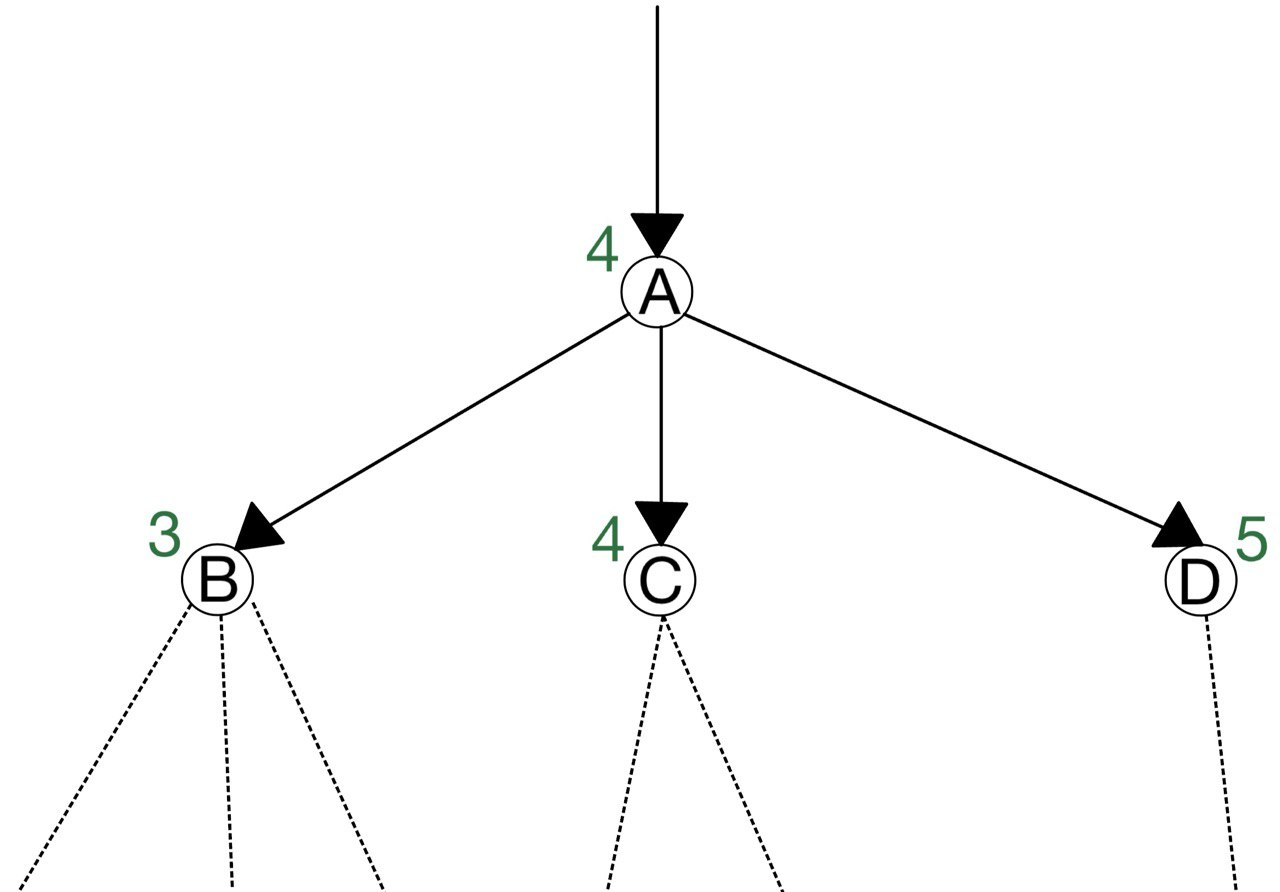
\includegraphics[scale=0.15]{figures/treeRoutingExample.jpg}}
    \caption{Example of Tree Routing used in step \fbox{4}. \textcolor{green}{Ranks} of the nodes.}

    \label{treeRoutingExample}
\end{figure}

\section{Evaluation}
\label{evaluation}

The evaluation is divided into two sections. First, in Fig. \ref{regulartopofig}, randomly generated graphs with randomized errors are evaluated. Subsequently, TopologyZoo \cite{topologyZoo} graphs with clustered errors are evaluated in Fig. \ref{realtopofig}.
We use Python to perform these graph-based simulations.
The metrics used in all figures are listed below:

$Hops$: the number of edges needed to reach a specific destination from a source. The average number of hops is calculated by summing the hops of all repetitions of a failure rate (or a graph in the case of Fig. \ref{realtopofig}) that did not fail, and then dividing by the number of repetitions of a failure rate that did not fail.

$Resilience$: the probability of success with which a packet reaches its destination from a source. To determine the average resilience, the following calculation is used. The sum of all resiliences of a failure rate (or a graph in the case of Fig. \ref{realtopofig}) is divided by the total number of repetitions for that failure rate.

In the following Section~\ref{randomEval}, each step on the X-axis represents the average of the results from 100 experimental runs for that value. In Section~\ref{realEval}, each step on the X-axis represents the average of the results from 5 experimental runs for that value. In each experimental run, the $s$ from which the packet is routed to $d$ changes. While $s$ changes in every run, $d$ remains the same for all runs at the current step on the X-axis. This approach provides 5 test runs for each step on the X-axis, using 5 different $s$ to route to the same $d$.

\subsection{Randomly Generated Graphs}
\label{randomEval}
First, the results of the randomized graphs from Fig.~\ref{regulartopofig} are evaluated. These graphs consist of 50 nodes, each with a connectivity of 5 or 8 respectively. In both plots, the respective metrics in relation to the failure rate can be seen. 
The first failure rate (FR) step involves selecting 5 edges uniformly at random from the total set of edges and marking them as faulty.
A FR step indicates that an additional 5 faulty edges are randomly selected, in the same manner as the first step, and added to the existing faulty edges.
The randomly generated graphs of this chapter are created by using the $random\_regular\_graph(n, k, seed)$ algorithm of NetworkX~\cite{networkx}, which generates a random
$k$-regular graph on $n$ nodes. For this experiment 100 $5$-regular and 100 $8$-regular graphs were generated. For each graph a destination
and five different starting points are chosen at random.

Additionally, one other algorithm from a recent paper~\cite{tree} is compared to the algorithm of this work. $OneTree$ is the original form, which operates without face routing and the checkpoint.

Regarding resilience, both algorithms offer maximum resilience up to FR=7 on $5$-regular graphs (FR=15 on $8$-regular), as can be seen in the left plot of Fig.~\ref{regulartopofig}.
From FR=8 on $5$-regular graphs (FR=16 on $8$-regular), $One Tree Checkpoint$ consistently achieves the highest resilience values.

Upon examining the hop counts in the right plot of Fig. \ref{regulartopofig}, it becomes apparent that $OneTree$ achieves an identical number of hops up to FR=6 on $5$-regular graphs (FR=11 on $8$-regular graphs). Starting from FR=7 on $5$-regular graphs, the hop counts of $OneTree$ exceed those of $OneTreeCheckpoint$.
On $8$-regular graphs between FR=11 and FR=24, the $OneTree$ Algorithm generally has a higher hop count than the $One Tree Checkpoint$, from FR=25 to FR=30, the $One Tree$ needs a smaller number of hops.

In summary, this means that, with regard to randomized regular graphs, the resilience is generally improved by the hybrid approach of this work but also requires a comparatively higher number of hops in some cases.

\begin{figure}[t]
    \centering
    \raisebox{0pt}[\height][\depth]{\hspace*{-1em}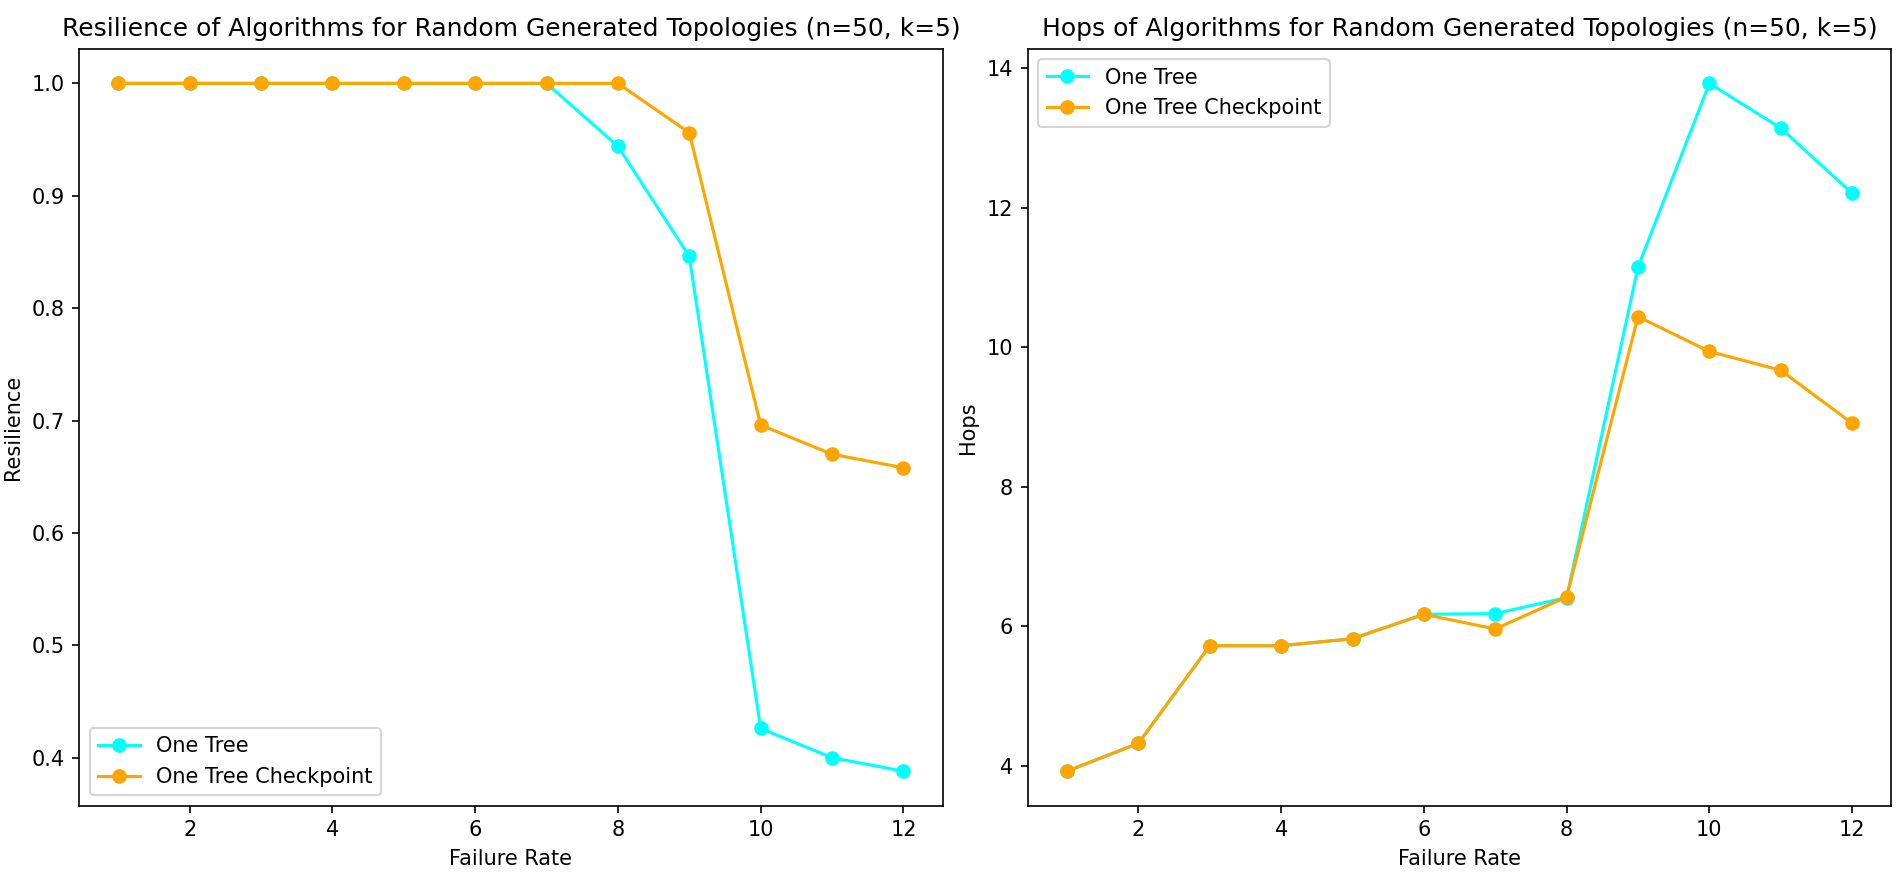
\includegraphics[scale=0.1, width=\linewidth]{figures/k5.png}}\\
    \raisebox{0pt}[\height][\depth]{\hspace*{-1em}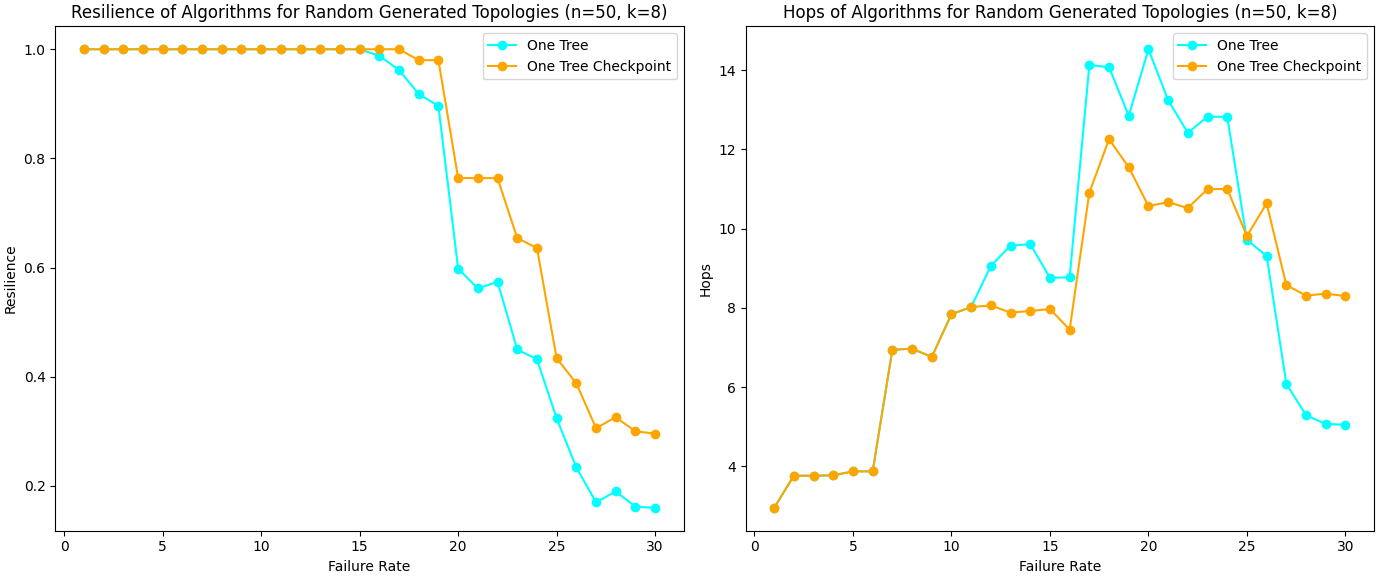
\includegraphics[scale=0.1, width=\linewidth]{figures/k8.png}}
    \caption{Comparison of the resilience and hops of different algorithms on randomly generated $5$-regular (upper) and $8$-regular (lower) graphs. 
    Each Failure Rate step represents an increment of 5 failures added to the network topology. The left plot displays the resilience (success rate) of each algorithm, while the right plot shows the average number of hops required.}
    \label{regulartopofig}
\end{figure}

% https://ieeexplore.ieee.org/stamp/stamp.jsp?tp=&arnumber=9488782 
% Seite 6

\subsection{Real World Graphs}
\label{realEval}
The experiments with the $OneTree$ and $OneTreeCheckpoint$ algorithms on real-world graphs~\cite{topologyZoo} are shown in Fig. \ref{realtopofig}. There, four graphs are listed with their number of nodes and measured hops/resilience. 
The used topologies consist of: $BtEurope$ with $n=24$, $Geant2001$ with $n=27$,  $Bics$ with $n=33$ and $Garr201105$ with $n=59$.
The chosen model for the clustered selection of faulty edges is taken from \cite{clusteredFailures}. 
This targeted attacks failure model simulates adversarial failures, such as those caused by attacks, by focusing on well-connected regions or clusters in the network. 
These clusters could represent strategically important areas, like groups of cities. 
An adversary might target links within these clusters to disrupt the network's fast-recovery capabilities.
In this model, links are selected for failure based on the clustering coefficient of nodes, with a predefined number of links either chosen randomly from a candidate set or fully disabled if the set contains fewer links than the failure parameter.

In the upper plot of Fig.~\ref{realtopofig}, it can be seen that $OneTreeCheckpoint$ achieves higher resilience in two out of the four experiments. This is due to the fact that this algorithm provides multiple entry points from the source, even when influenced by several faulty edges.
However, it can also be observed that $OneTree$ delivers increased resilience values in the experiments with graphs of $n=24$ and $n=59$. This can be attributed to the fact that, in selected cases, expanding a single EDP is more effective than creating a broader hybrid structure.
Considering the hops in the lower plot of Fig.~\ref{realtopofig}, both algorithms achieve similar numbers in the first three experiments. 
In the fourth experiment, a significant increase in hops is observed for $OneTreeCheckpoint$, which can be attributed to the structure of the hybrid architecture having a larger number of edges. However, in selected cases, this also leads to substantial overhead regarding the hop count.

It is also noteworthy that the precomputation time of the algorithms was measured in the experiments, although not graphically represented. From these results, it can be concluded that $OneTreeCheckpoint$ typically requires three times as much time as the $OneTree$ algorithm needs for precomputation.

In summary, it can be concluded that $OneTreeCheckpoint$ enhances resilience by approximately 10.64\%, making it more adept at withstanding clustered failures. However, in some cases, the increased hops due to its larger structure may lead to unnecessary overhead, potentially compromising its resilience despite these improvements.

\begin{figure}[t]
    \centering
    \raisebox{0pt}[\height][\depth]{\hspace*{-1em}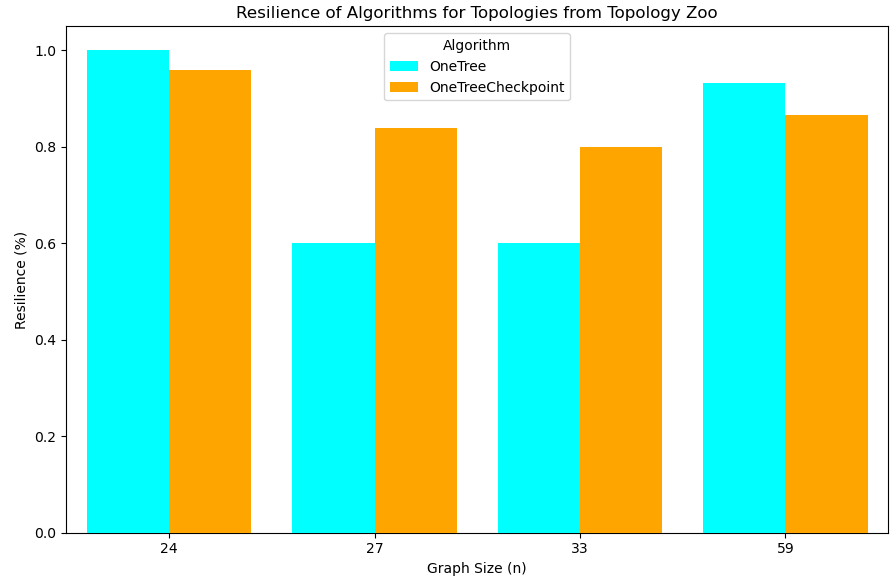
\includegraphics[scale=0.3]{figures/realTopoAfterChange_left.png}}\\
    \raisebox{0pt}[\height][\depth]{\hspace*{-1em}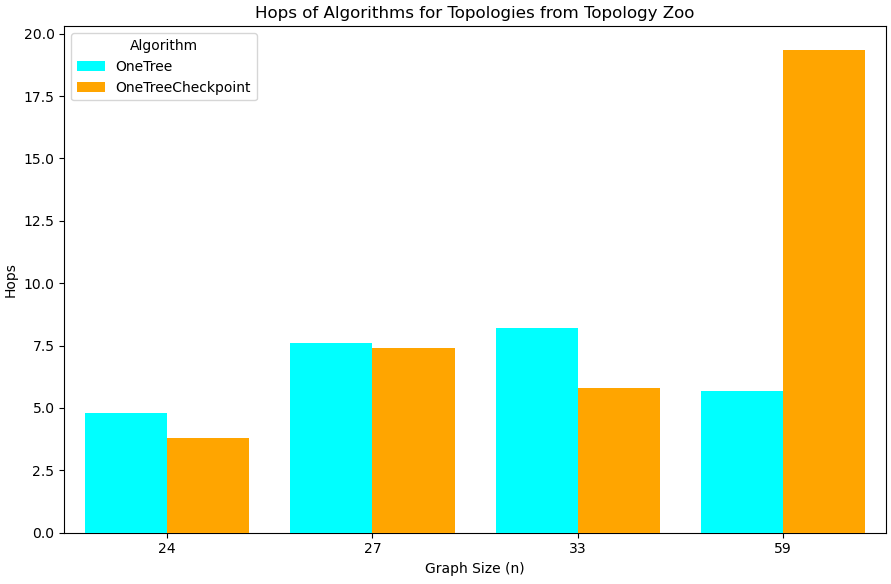
\includegraphics[scale=0.3]{figures/realTopoAfterChange_right.png}}
    \caption{Comparison of the resilience and hops of the two algorithms on various graph sizes using topologies from the Topology Zoo. The upper plot shows the resilience (success rate) of each algorithm, while the lower plot illustrates the average number of hops. Each bar represents the aggregated results from 5 experimental runs.}
    \label{realtopofig}
\end{figure}




\section{Conclusion}\label{conclusion}
%Nochmal kurz was ich gemacht habe.
This work presents an initial approach to combine the advantages of face routing with those of tree routing. Initially, packets are forwarded from the source to a checkpoint $cp$ via face routing. 
Next, the packets reach their destination with the help of tree routing. 
This method was chosen to counteract clustered failures at the source and to provide a variety of entry points into the routing for the packets.
%Was dabei rausgekommen ist.
%The evaluation of this method was described in Section \ref{evaluation}. 
It has been observed that the hybrid approach can enhance resilience not only in the case of clustered failures but also in comparison to similar algorithms in scenarios involving random failures.
%Das man das auch noch verbessern könnte.
%Furthermore, additional suggestions for improvement and modifications were mentioned in Section \ref{outlook}, which should serve as incentives for future work.

\section{Outlook}
\label{outlook}
Subsequently, further possibilities are described for improving the combination of face routing and tree routing.
One possibility is to modify the choice of $cp$ by, for example, already globally knowing the "fault tolerance" of a node and thus highlighting it in the choice of $cp$. This choice can also be randomized in other ways.
Another approach could be to modify the tree formation. Modifications could be incorporated, such as building multiple trees or restricting the width of the tree. However, in this case, it would be necessary to evaluate whether the graph is large enough to fill multiple trees.
Furthermore, in some scenarios, it would be beneficial to use multiple $cp$, through which routing should be performed.



%%
%% Bibliography
%%

%% Please use bibtex, 
\balance
\bibliographystyle{IEEEtran}
\bibliography{IEEEbib}

\end{document}
